\documentclass[twocolumn]{article} %formato
\usepackage{graphicx} % graficos
\usepackage{amsmath} %matrices
\usepackage{float}    
\usepackage{hyperref}


\graphicspath{{Imagenes/}} %graficos

\usepackage[spanish]{babel} %idioma


\spanishdecimal{.}
\setlength{\parskip}{1em} 

\begin{document}

\title{Determinación de la constante de Boltzmann mediante la caracterización eléctrica de un diodo}
\author{Jesús Armando Cañas y Miguel Angel Perdomo}
\date{\today}


\maketitle

\begin{abstract}
   El presente artículo se propone calcular la constante de Boltzmann empleando una relación que existe entre los diodos y esta constante. Inicialmente, en aumentos de 0.01 voltios, se midieron el voltaje y la corriente del circuito, se realizó una prueba de bondad de ajuste de la curva exponencial obtenida y, a partir de este ajuste, se calculó la constante y su incertidumbre. Se hizo lo mismo en aumentos de 0.05 voltios, se repitió el proceso tres veces, se linealizó el ajuste y se obtuvo la constante. Finalmente, el caso de aumentos de 0.01 voltios fue el más cercano al valor aceptado.
\end{abstract}

\vspace{2cm} 

\section{Introducción}
\vspace{-0.3cm}
La constante de Boltzmann ($k_B$) posee diversas aplicaciones en la física estadística y la termodinámica, dado que establece el vínculo fundamental entre la energía microscópica y la temperatura macroscópica. Esta constante fue determinada por primera vez en 1901 por Max Planck en su formulación de la ley de la radiación del cuerpo negro \cite{Planck1901}. Con anterioridad a 2018, su valor se obtenía de manera experimental y contaba con una incertidumbre asociada; sin embargo, con la revisión del Sistema Internacional de Unidades (SI) en dicho año, su valor se fijó de manera exacta en $1.380\,649\times 10^{-23} J/K$\cite{Stock2019}.

Existen múltiples sistemas físicos donde la constante de Boltzmann emerge de forma natural. Un caso particular de especial interés es el diodo semiconductor. Este dispositivo está compuesto por la unión de dos materiales semiconductores (tipo P y tipo N), configuración que permite el flujo de corriente mayoritariamente en una sola dirección. El montaje experimental analizado consta de una fuente de voltaje de alta precisión, una resistencia y un diodo. En este tipo de circuitos, la relación entre la corriente ($I$) y el voltaje ($V$) sigue un comportamiento exponencial que se explicará con más detalle en el marco teórico ~\cite{leon2014}.

El propósito de este artículo es determinar experimentalmente la constante de Boltzmann. A partir del circuito mencionado, y conociendo parámetros como la temperatura, la carga del electrón y el factor de idealidad, se puede realizar un ajuste exponencial a los datos de corriente y voltaje para despejar $k_B$. Específicamente, al variar el voltaje aplicado se obtiene un conjunto de puntos experimentales ($V, I$) sobre los cuales se aplica un método de ajuste, permitiendo así extraer el valor de la constante a partir de los coeficientes del ajuste obtenido.


\section{Marco teórico}
\subsection{Bondad de ajuste y test de hipótesis}

Inicialmente, una hipótesis es aquella suposición que se plantea respecto a alguna población o problema con el fin de verificar su veracidad o falsedad. Adicionalmente, una hipótesis nula $H_0$ es aquella hipótesis que inicialmente se asume como cierta con la finalidad de verificarla o falsarla, y la hipótesis alternativa $H_a$ será una suposición que sea contraria a la hipótesis nula. Cabe aclarar que tanto la hipótesis nula como la alternativa deben ser mutuamente excluyentes (contrarias entre sí). Se le llama test de hipótesis a aquel proceso mediante el cual se busca aceptar o rechazar la hipótesis nula. Sin embargo, cabe añadir que este es un proceso probabilístico y no absoluto; por lo cual, que la hipótesis nula sea verdadera o falsa no es un hecho inequívoco. Para poder verificar o falsar la hipótesis nula, existen múltiples herramientas, como la llamada \textit{prueba de bondad de ajuste}, con la cual podemos determinar si ciertos datos experimentales se ajustan a una distribución determinada \cite{marques1991probabilidad}.
\subsection{Distribución chi-cuadrado}

Si se considera que ciertos datos siguen una distribución determinada, se puede establecer que un evento $E_k$ ocurre con una frecuencia observada $O_k$. Según la distribución teórica, los datos siguen una frecuencia esperada $e_k$; luego, $\chi^2$ se define como \cite{marques1991probabilidad}:

\begin{equation}
\chi^2 = \sum_{k=1}^{n} \frac{(O_k - e_k)^2}{e_k} 
\label{chi}
\end{equation}

Finalmente, tras obtener el estadístico de la distribución chi-cuadrado, es necesario considerar cómo se va a concluir y bajo qué condiciones se determinará que la hipótesis nula se cumple. Así, se define el nivel de significancia ($\alpha$) como la probabilidad de rechazar la hipótesis nula aunque esta sea cierta. Usualmente, en física experimental se emplea un nivel de significancia igual al 5\% \cite{marques1991probabilidad}.

\subsection{Incertidumbres pequeñas} \label{Inceridumbres pequeñas}
Sea $x$ una variable aleatoria, tal que $x=f(u,v,\dots)$. Luego, su varianza $\sigma_x^2$ se puede determinar como~\cite{bevington2003data}:

\begin{equation}
    \sigma_x^2=\sigma_u^2\left(\frac{\partial x}{\partial u}\right)^2 + \sigma_v^2\left(\frac{\partial x}{\partial v}\right)^2 + \dots + 2\sigma_{uv}^2\left(\frac{\partial x}{\partial u}\right)\left(\frac{\partial x}{\partial v}\right)
\end{equation}

Si las variables de $f$ son independientes, el término $2\sigma_{uv}^2\left(\frac{\partial x}{\partial u}\right)\left(\frac{\partial x}{\partial v}\right)=0$. Luego, la expresión para determinar la varianza sería la siguiente~\cite{bevington2003data}:

\begin{equation}
    \sigma_x^2=\sigma_u^2\left(\frac{\partial x}{\partial u}\right)^2 + \sigma_v^2\left(\frac{\partial x}{\partial v}\right)^2 + \dots
\end{equation}
\subsection{Incertidumbre estándar y efectiva}
Si se repite $n$ veces la medición de una variable aleatoria de una distribución, puede calcularse la incertidumbre estándar como~\cite{marques1991probabilidad}:

\begin{equation}
    \sigma_{\bar{x}} = \frac{\sigma}{\sqrt{n}}
\end{equation}

Si tenemos una función $y=f(x)$ y contamos con una incertidumbre $\sigma_x$ en la variable independiente, se puede propagar la incertidumbre a la variable dependiente por medio de la siguiente ecuación~\cite{bevington2003data}:

\begin{equation}
    \sigma_y^2 = \sigma_x^2 \left( \frac{\partial y}{\partial x} \right)^2 + \sigma_{yD}^2
\end{equation}

El primer término corresponde a la incertidumbre asociada a la variable independiente y el segundo a la incertidumbre intrínseca de la variable dependiente~\cite{bevington2003data}.

\subsection{Error porcentual }
Si se tiene un valor aceptado de una constante ($v_a$) y un valor experimentalmente obtenido ($v_e$), el error porcentual $\epsilon_{\%}$ se determina como~\cite{JCGM2008}:

\begin{equation}
    \epsilon_{\%} = \frac{|v_a - v_e|}{v_a} \times 100\%
\end{equation}
\subsection{Grados de libertad y valor crítico}
Los grados de libertad de una distribución pueden calcularse como~\cite{sirca2016probability}:
\begin{equation}
    \nu = n - m - 1 
    \label{nu}
\end{equation}
Donde cada término se define de la siguiente manera:

\begin{itemize}
    \item[$n$:] Número de clases o bines independientes en los que se han agrupado los datos del histograma.
    \item[$m$:] Número de parámetros que no son conocidos a priori y que se estiman mediante los datos obtenidos experimentalmente~\cite{sirca2016probability}.
\end{itemize}

Por otro lado, el valor crítico se define como aquel umbral tal que, si el estadístico chi-cuadrado es mayor que dicho valor, se rechaza la hipótesis nula; de lo contrario, si es menor, la hipótesis nula es aceptada. A partir del nivel de significancia, se puede calcular el valor crítico ($x_*$) como~\cite{sirca2016probability}:

\begin{equation}
    \alpha = \int_{x_*}^{\infty} f(x; \theta_0) \, dx 
\end{equation}

Donde:
\begin{itemize}
    \item[$x_*$:] Valor crítico.
    \item[$f(x;\theta)$:] Función de densidad de probabilidad del estadístico de prueba bajo la hipótesis nula, caracterizada por el parámetro $\theta$.
    \item[$\alpha$:] Nivel de significancia.
\end{itemize}



\subsection{Método de mínimos cuadrados}

El método de mínimos cuadrados es un procedimiento utilizado para ajustar una recta a un conjunto de datos, de tal manera que la suma de los cuadrados de los residuos (las diferencias entre los valores observados y los valores estimados) sea mínima.

Sea un conjunto de datos $(x_i, y_i)$ para $i = 1, 2, \dots, n$, se desea encontrar la recta de regresión:

\begin{equation}
    y = a + bx
\end{equation}

donde $a$ es la ordenada al origen y $b$ es la pendiente. La recta se determina minimizando la función de error:

\begin{equation}
    S = \sum_{i=1}^{n} (y_i - a - bx_i)^2
\end{equation}

Al derivar parcialmente respecto a $a$ y $b$ e igualar a cero, se obtienen las ecuaciones normales:

\begin{align}
    \sum y_i &= na + b \sum x_i \\
    \sum x_i y_i &= a \sum x_i + b \sum x_i^2
\end{align}

Resolviendo este sistema, se obtienen los estimadores:

\begin{equation}
    b = \frac{n \sum x_i y_i - \sum x_i \sum y_i}{n \sum x_i^2 - (\sum x_i)^2}
\end{equation}

\begin{equation}
    a = \bar{y} - b \bar{x}
\end{equation}

donde:

\begin{equation}
    \bar{x} = \frac{1}{n}\sum x_i, \quad \bar{y} = \frac{1}{n}\sum y_i
\end{equation}

La recta obtenida se denomina recta de regresión de $Y$ sobre $X$~\cite{marques1991probabilidad}.


\subsection{Matriz de Covarianza}\label{covarianza}
La covarianza es una medida que indica el grado en que dos variables aleatorias varían conjuntamente.

Para dos variables aleatorias $X$ y $Y$, la covarianza se define como:

\begin{equation}
\mathrm{Cov}(X,Y) = E[(X - \mu_X)(Y - \mu_Y)]
\end{equation}

donde $\mu_X$ y $\mu_Y$ son las medias de $X$ y $Y$, respectivamente.

Para un conjunto de datos muestrales, la covarianza se calcula mediante la siguiente expresión:

\begin{equation}
\mathrm{Cov}(X,Y) = \frac{1}{n} \sum_{i=1}^{n} (x_i - \bar{x})(y_i - \bar{y})
\end{equation}

La matriz de covarianza para un vector aleatorio $\mathbf{X} = (X_1, X_2, \dots, X_p)$ se define como:

\begin{equation}
\begin{pmatrix}
\mathrm{Var}(X_1) & \mathrm{Cov}(X_1,X_2) & \cdots & \mathrm{Cov}(X_1,X_p) \\
\mathrm{Cov}(X_2,X_1) & \mathrm{Var}(X_2) & \cdots & \mathrm{Cov}(X_2,X_p) \\
\vdots & \vdots & \ddots & \vdots \\
\mathrm{Cov}(X_p,X_1) & \mathrm{Cov}(X_p,X_2) & \cdots & \mathrm{Var}(X_p)
\end{pmatrix}
\end{equation}

donde los elementos de la diagonal representan las varianzas y los elementos fuera de la diagonal representan las covarianzas.

Esta matriz es simétrica y juega un papel fundamental en el análisis multivariado y en la teoría de regresión~\cite{marques1991probabilidad}.
\subsection{Diodos}

\subsubsection{Semiconductores}
Los semiconductores son elementos cuyas propiedades conductivas oscilan entre las de un elemento conductor y un aislante. Por lo general, hay dos tipos de materiales semiconductores: de un solo cristal y compuestos. Los semiconductores de un solo cristal, como el germanio (Ge) y el silicio (Si), tienen una estructura cristalina repetitiva, en tanto que compuestos como el arseniuro de galio (GaAs), el sulfuro de cadmio (CdS), el nitruro de galio (GaN) y el fosfuro de galio y arsénico (GaAsP) se componen de dos o más materiales semiconductores de diferentes estructuras atómicas~\cite{rosadio}.

\subsubsection{Clasificación de los semiconductores}
Los semiconductores se clasifican en dos tipos:
\begin{enumerate}
    \item \textbf{Semiconductor tipo $n$}: son los semiconductores en los que hay un exceso de electrones libres comparados con el número de huecos. Es por esto que se le atribuye el nombre $n$, por el carácter negativo~\cite{rosadio}.
    \item \textbf{Semiconductores tipo $p$}: en este tipo de semiconductores hay un exceso de huecos comparado con el número de electrones libres. Los elementos más utilizados para este propósito son el boro, galio e indio. El término $p$ se atribuye refiriéndose al positivo~\cite{rosadio}.
\end{enumerate}

\subsubsection{Unión $p-n$, composición del diodo}
Cuando se dopa un material semiconductor de modo que una mitad sea tipo $p$ y la otra de tipo $n$, se forma lo que denominamos un diodo semiconductor; el borde entre la zona de tipo $p$ y la zona de tipo $n$ se denomina unión $p-n$~\cite{rosadio}.

\subsubsection{Clasificación de los tipos de diodo}

\begin{itemize}

\item \textbf{Polarización directa}\newline
Un diodo tiene polarización directa cuando se conecta un terminal positivo al material de tipo $p$ y un terminal negativo al material de tipo $n$, tal como se muestra en la figura \ref{directa}.

\begin{figure}[ht]
    \centering
    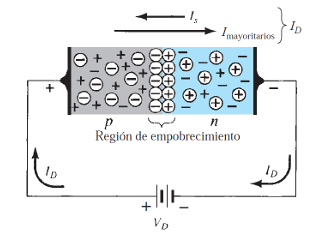
\includegraphics[width=1.0 \linewidth]{diodo con polarizacion directa.png}
    \caption{Diodo con polarización directa}
    \label{directa}
\end{figure}

En este caso de polarización directa, los electrones y huecos son empujados hacia la unión. Si la tensión entre terminales es menor que la barrera de potencial, los electrones libres de la zona $n$ no tienen la suficiente energía para atravesar la zona de deplexión. Cuando entran en esta zona, los iones se ven empujados de vuelta a la región $n$, por lo que no circula corriente a través del diodo. Cuando la tensión entre terminales es mayor que la barrera de potencial, se empuja de nuevo a huecos y electrones libres hacia la unión. En este caso, existe un flujo de electrones de la parte de material $n$ a la parte de material $p$~\cite{rosadio}.

\item \textbf{Polarización inversa}\newline
Un diodo tiene polarización inversa si se le conecta una terminal negativa a la parte del material tipo $p$ y el terminal positivo a la parte tipo $n$ (figura \ref{inversa}).

\begin{figure}[ht]
    \centering
    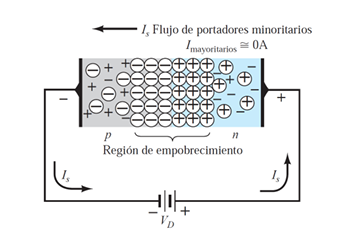
\includegraphics[width=1\linewidth]{diodo con polarizacion inversa.png}
    \caption{Diodo con polarización inversa}
    \label{inversa}
\end{figure}

\end{itemize}

Aquí, los huecos son atraídos por el terminal negativo, mientras que los electrones libres son atraídos por el positivo. Esto origina que los electrones libres y los huecos se alejen de la unión y, a medida que se alejan, dejan tras su paso iones positivos y negativos respectivamente, originando un ensanchamiento de la zona de deplexión. Esta crea una barrera demasiado grande para que los portadores mayoritarios la puedan superar, por lo que el flujo de estos se reduce a cero. Sin embargo, el número de portadores minoritarios que entran a la zona de deplexión no cambia, y se producen vectores de flujo de portadores minoritarios de la misma magnitud~\cite{rosadio}.

La corriente en la polarización inversa se denomina corriente de saturación; el término saturación se deriva del hecho de que no cambia significativamente con los cambios de potencial proporcionados al circuito eléctrico. Por otro lado, el comportamiento de la corriente en función del voltaje, una vez se supera la barrera de potencial, se puede modelar por~\cite{leon2014}:

\begin{equation}
I = I_s \left( e^{\frac{qV}{\eta k_B T}} - 1 \right)
\label{corriente}
\end{equation}

Donde:
\begin{itemize}
    \item $I_s$ es la corriente de saturación,
    \item $q$ es la carga del electrón,
    \item $V$ es el voltaje aplicado al diodo,
    \item $\eta$ es el coeficiente de idealidad,
    \item $k_B$ es la constante de Boltzmann,
    \item $T$ es la temperatura absoluta.
\end{itemize}

\subsection{Relación de la constante de Boltzmann en circuitos con diodos}

En los circuitos con diodos, la constante de Boltzmann $k_B$ juega un papel fundamental en la descripción del transporte de carga, particularmente en la ecuación característica corriente-voltaje del diodo. La constante de Boltzmann aparece a través del denominado \textbf{voltaje térmico}, definido como:

\begin{equation}
V_T = \frac{k_B T}{q}
\end{equation}

Este voltaje térmico determina la escala a la cual la temperatura afecta el comportamiento del diodo. La presencia de $k_B$ en la ecuación del diodo refleja que el transporte de portadores está gobernado por procesos térmicos. Específicamente~\cite{leon2014}:

\begin{itemize}
    \item Controla la energía térmica disponible para que los electrones superen la barrera de potencial.
    \item Determina la generación de portadores minoritarios.
    \item Influye en la corriente de saturación y en la conducción en polarización inversa.
\end{itemize}

Adicionalmente, el valor definido por el Sistema Internacional para la constante de Boltzmann $k_B$~\cite{Stock2019} es de:
\begin{equation}
    k_B = 1.380\,649 \times 10^{-23} \, \text{J/K}
    \label{kb}
\end{equation}
\section{Metodología}

\subsection{Montaje}
Se empleó el circuito que se muestra a continuación:

\begin{figure}[ht]
    \centering
    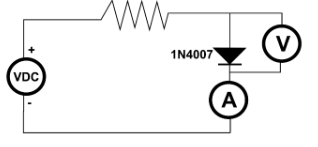
\includegraphics[width=0.7\linewidth]{circuito.png}
    \vspace{0.5cm} 
    \caption{Foto del circuito a montar.}
    \label{fig:sistema}
\end{figure}

Inicialmente, se armó el circuito de la figura \ref{fig:sistema}. Posteriormente, se colocó una fuente que permitiera aumentar el voltaje en pequeños pasos con precisión. El montaje se presenta en las figuras \ref{fig:termómetro} y \ref{fig:circuito}:

\begin{figure}[ht]
    \centering
    \includegraphics[width=0.7\linewidth]{Montaje.jpg}
    \caption{Circuito del experimento.}
    \label{fig:circuito}
\end{figure}

\begin{figure}[H]
    \centering
    \includegraphics[width=0.7\linewidth]{termometro montaje 2.jpg}
    \caption{Termómetro que registró la medida de temperatura.}
    \label{fig:termómetro}
\end{figure}

Se puede observar a la izquierda de la Figura \ref{fig:circuito} la fuente empleada durante el experimento. En la parte central, se observa el circuito de la Figura \ref{fig:sistema} y, a la derecha, los dos multímetros utilizados: uno para el voltaje y otro para la corriente. En la figura \ref{fig:termómetro} se puede observa el termómetro empleado para determinar la temperatura y la termocupla que este emplea.

\subsection{Metodología}

Se comenzó con un voltaje inicial de $0.3$ V para el primer muestreo. Luego, se aumentó el voltaje en intervalos de $0.01$ V. Posteriormente, se registraron los datos de corriente y voltaje para aproximadamente 100 medidas.

Para las siguientes muestras, se inició en $0.3$ V y se aumentó el voltaje en intervalos de $0.05$ V. Además, se registraron los datos de voltaje y corriente proporcionados por los multímetros hasta que la medida de voltaje del diodo fuese cercana a $0.7$ V. Este procedimiento se repitió tres veces.

En el análisis de los datos, para aquellos obtenidos con pasos de $0.01$ V, se realizó un ajuste exponencial de la forma:
\begin{equation}
    I(V) = a e^{bV}
    \label{exponencial}
\end{equation}

Después de ejecutado el ajuste, se aplicó el test de $\chi^2$ para verificar la bondad del ajuste. Se toma a $H_0$ como: \textit{La muestra presenta un comportamiento exponencial de la forma \ref{exponencial}}, y a $H_a$ como: \textit{La muestra no presenta un comportamiento exponencial de la forma \ref{exponencial}}. Nuevamente, si el $\chi^2$ obtenido es menor que el valor crítico, se acepta $H_0$; de lo contrario, se rechazará. Como $H_0$ fue respaldada, se pudo usar la siguiente relación al despejar e igualar el coeficiente del exponente de las ecuaciones (\ref{corriente}) y (\ref{exponencial}):

\begin{equation}
b = \frac{e}{\eta k_B T}
\end{equation}

A partir de $b$, se puede encontrar la constante $k_B$ conociendo la temperatura $T$ del ambiente y sabiendo que el coeficiente de idealidad posee un valor $\eta = 1.91$ y la carga del electrón $e = 1.602176634\times10^{-19}$ C~\cite{Stock2019}. En consecuencia:

\begin{equation*}
    k_B = \frac{e}{\eta b T}
    \label{Valor: kb}
\end{equation*}

Para el valor de $k_B$ se calculó la incertidumbre por incertidumbres pequeñas, sabiendo que la incertidumbre de $b$ es uno de los elementos de la diagonal de la matriz de covarianza (ver \ref{covarianza}) y conociendo la incertidumbre de $T$. También se calculó el error porcentual.

Aplicando $\ln$ a ambos lados de la igualdad de la ecuación (\ref{exponencial}):
\[ \ln(I) = \ln(a e^{bV}) \]

Se obtiene:
\begin{equation}
     \ln(I) = \ln(a) + bV
     \label{lin}
\end{equation}

Para los datos tomados con pasos de $0.05$ V, se realizó una linealización de los datos siguiendo la ecuación (\ref{lin}) mediante la librería \texttt{scipy.optimize} de Python. Luego, se calculó el coeficiente $R^2$ para comprobar la bondad del ajuste, ya que no se puede aplicar el test de bondad de $\chi^2$ debido a que, al realizar una transformación de los datos operando con $\ln$, no se conserva la forma mostrada en (\ref{chi}). Es decir, existe un sesgo en el análisis por el cual no se pueden comparar datos de una métrica de escala con otra diferente, más aún cuando la transformación logarítmica no es lineal.

Si $R^2$ es cercano a 1, se hereda el mismo $b$ para encontrar la constante de Boltzmann. Así, para calcular $k_{B,i}$ de las tres muestras, se emplea la misma ecuación (\ref{kb}); la incertidumbre de los $k_{B,i}$ se calcula de la misma manera que en el procedimiento anterior. Luego, se promedian los valores $k_{B,i}$ obtenidos y se calcula la desviación estándar. Al final, se reporta el valor de $k_B$ obtenido con incertidumbre efectiva y error porcentual.

Por último, se discuten las posibles fuentes de error, se considera cuál de los dos procedimientos es mejor para obtener el valor de $k_B$ y se debate por qué no se empleó el test de hipótesis de chi-cuadrado en el segundo ajuste.

\section{Resultados}

\subsection{Medidas por intervalos de 0.01 V}

El ajuste obtenido para las medidas tomadas por intervalos de $0.01$ V se muestra en la Figura \ref{0.01}.

\begin{figure}[ht]
    \centering
    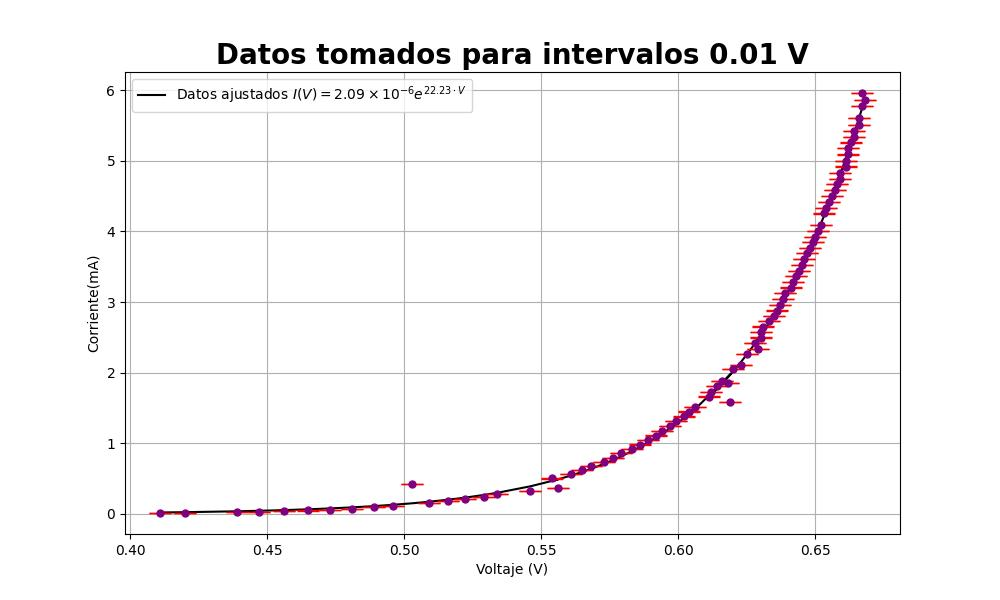
\includegraphics[width=1\linewidth]{Imagenes/datos_0.01.jpg}
    \caption{Gráfica correspondiente al ajuste exponencial para los datos tomados por intervalos de 0.01 V.}
    \label{0.01}
\end{figure}

En el eje $x$ se encuentra el voltaje (variable independiente) y en el eje $y$ se encuentra la corriente (variable dependiente). Los puntos experimentales obtenidos sugieren una relación exponencial, lo cual se confirma con el tipo de ajuste obtenido (curva negra). El ajuste visualmente es correcto; no obstante, para garantizar una correcta argumentación, se debe proceder con el testeo y análisis de incertidumbre.

\begin{equation}
    \begin{pmatrix}
4.3\times10^{-14} & -3.1\times10^{-8} \\
-3.1\times10^{-8} & 2.3\times10^{-2}
\end{pmatrix}
\label{cov01}
\end{equation}

En (\ref{cov01}) se muestra la matriz de covarianza para el ajuste. El segundo elemento de la diagonal corresponde a la varianza del parámetro $b$. De la matriz de covarianza se puede verificar que los valores que no pertenecen a la diagonal son muy cercanos a cero, lo que expresa la independencia entre los parámetros $a$ y $b$.

Así, el valor de este parámetro con su respectiva incertidumbre es:
\begin{equation*}
 b = 22.23 \pm 0.02
\end{equation*}

Usando el test de hipótesis de $\chi^2$ para comprobar la bondad del ajuste, con un nivel de significancia del $5\%$, para $\nu = 2$ grados de libertad y acorde a la ecuación (\ref{nu}), se obtuvo un valor crítico de $5.992$. Al comparar con el valor de $\chi^2 = 0.28$ obtenido en el ajuste, es posible respaldar la hipótesis nula y rechazar la hipótesis alternativa.

Usando el valor de $b$ para calcular la constante de Boltzmann $k_B$, se obtuvo que:
\begin{equation*}
k_B = (1.27 \pm 0.01) \times 10^{-23} \, \text{J/K}
\end{equation*}

La incertidumbre obtenida corresponde a la calculada por medio de incertidumbres pequeñas. Por otro lado, el error porcentual de la medida obtenida, en comparación con el definido por el Sistema Internacional de Unidades (\ref{kb}), es del $8\%$.

\subsection{Medidas por intervalos de 0.05 V}

En este caso, como fue indicado en la metodología, se linealizó la función exponencial (\ref{exponencial}) y se realizó un ajuste lineal para tres muestras de datos (Figura \ref{imagen0.05}). Luego, se verificó la bondad del ajuste usando el coeficiente $R^2$ de la teoría de mínimos cuadrados. En este caso no se empleó el test de hipótesis de chi-cuadrado pues, acorde a la ecuación (\ref{chi}), tanto la frecuencia observada ($O_k$) como la frecuencia teórica ($e_k$) deben estar en la misma métrica o en los mismos espacios de escala para ser comparadas. Al aplicar el logaritmo natural en la ecuación (\ref{exponencial}), se realiza una transformación a un espacio de escala logarítmica; al no estar en los mismos espacios de escala, una comparación mediante chi-cuadrado no sería coherente, ya que la transformación logarítmica no es lineal, lo que llevaría a un sesgo. Sobre esto se profundizará en el apartado de \textit{Conclusiones}.

\begin{figure}[H]
    \centering
    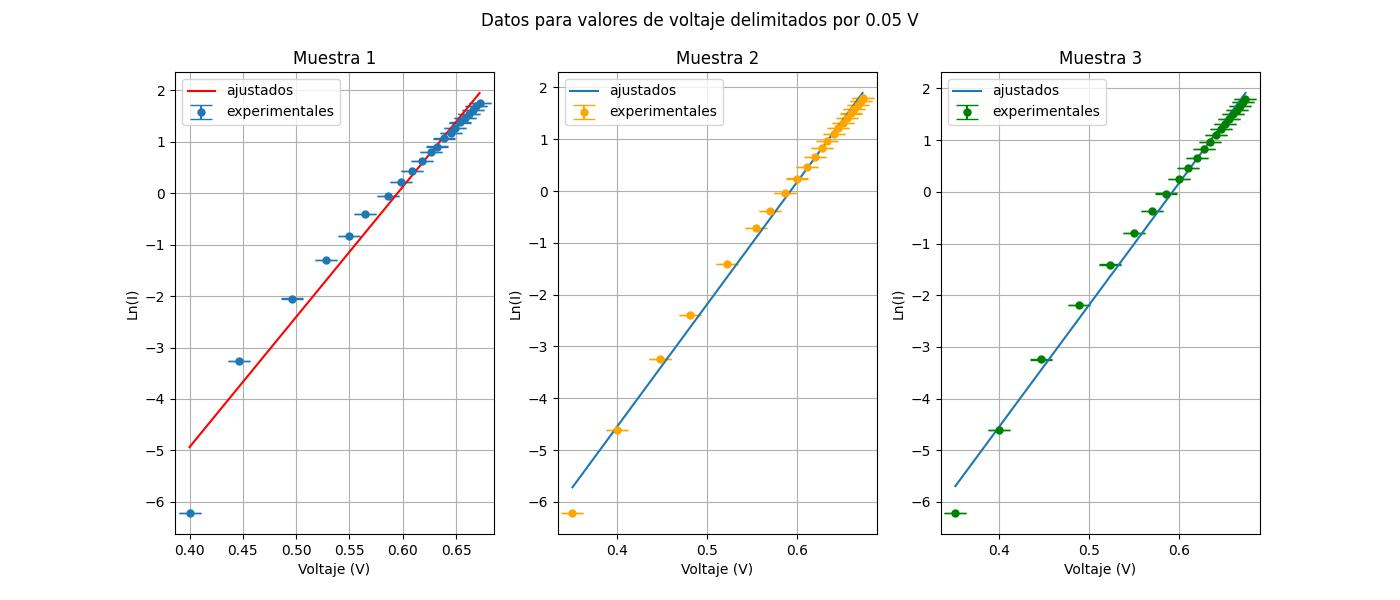
\includegraphics[width=1\linewidth]{Imagenes/datos_0.05.jpg}
    \caption{Gráficos obtenidos para la linealización de las medidas.}
    \label{imagen0.05}
\end{figure}

Los valores obtenidos de $R^2$ para los ajustes correspondientes a la Figura \ref{imagen0.05} son: 
\begin{equation*}
    0.96, \quad 0.99, \quad 0.99
\end{equation*}
Lo que indica que los tres ajustes predicen de manera correcta el comportamiento de los datos experimentales. Por otro lado, los valores obtenidos de $k_B$ con sus respectivas incertidumbres a partir del parámetro $b$ del ajuste lineal para cada muestra son:
\begin{itemize}
    \item Muestra 1: $(1.12 \pm 0.05) \times 10^{-23}$ J/K
    \item Muestra 2: $(1.20 \pm 0.02) \times 10^{-23}$ J/K
    \item Muestra 3: $(1.20 \pm 0.02) \times 10^{-23}$ J/K
\end{itemize}

Al promediar los datos de las medidas de $k_B$ y reportar la medida con incertidumbre efectiva, se obtiene:
\begin{equation*}
k_B = (1.17 \pm 0.03) \times 10^{-23} \, \text{J/K}
\end{equation*}

El error porcentual obtenido para la medida, comparado con el valor definido por el SI (\ref{kb}), es del $15\%$.

En el apéndice se puede encontrar el \textit{notebook} en el cual se trabajó para obtener los resultados expuestos.



\section{Conclusiones}

\begin{enumerate}
    \item En primer lugar, se obtuvo que, de las dos metodologías planteadas, la que demostró ser más precisa en la determinación de la constante de Boltzmann fue la del ajuste realizado con la función exponencial sin linealizar los datos. Con este procedimiento se consiguió un error porcentual de $\epsilon_{\%}=8\%$, en comparación con el segundo ajuste, el cual difiere del valor definido por el SI en un $15\%$.

    \item Si bien el primer ajuste difiere menos del valor de $k_B$ definido por el SI, debe considerarse que en este se contó con una mayor cantidad de datos; por lo cual, el ajuste representaría mejor el comportamiento físico, sumado al hecho de que la variación del voltaje fue menor. Esto implica que, independientemente de que se repitiera el segundo ajuste varias veces, no se mejoraría su calidad si intrínsecamente posee una resolución más pobre. Por tanto, una mejora metodológica consistiría en tomar la misma cantidad de datos para cada ajuste con idéntica variación del voltaje. Esto permitiría analizar cómo cambia el valor según el procedimiento (toma única vs. promedio de repeticiones) para compararlos equitativamente. Se requiere un diseño simétrico para concluir si la superioridad de un ajuste reside en su naturaleza matemática o en la densidad del muestreo.
    
    \item A partir de la matriz de covarianza, se determinó que los valores extradiagonales son muy cercanos a cero, lo que implica que los parámetros $a$ y $b$ son independientes entre sí. Esto significa que la incertidumbre de $b$ es aproximadamente independiente del resto de los parámetros; en consecuencia, no es estrictamente necesario calcular la incertidumbre de la corriente de saturación ($I_s$) para determinar la incertidumbre de $b$.
    
    \item En el primer ajuste, se demostró mediante el test de bondad de ajuste chi-cuadrado que la relación entre voltaje y corriente en un diodo sigue un comportamiento exponencial, tal como lo predice teóricamente la ecuación \eqref{exponencial}. Por otro lado, como se discutió en el apartado de resultados, no se empleó dicho test para el segundo procedimiento. Esto se debe a que la transformación no lineal del logaritmo altera el espacio métrico y crea un sesgo en el test, ya que se estarían comparando escalas con diferentes métricas que deformarían la interpretación estadística de forma no lineal. Por ende, se optó por el coeficiente $R^2$ para los ajustes lineales.
    
    \item Una posible fuente de error en la medición de la constante de Boltzmann fue la determinación de la temperatura, pues se registró la temperatura ambiente del laboratorio. Esta medida podría diferir de la temperatura interna de la unión del diodo o fluctuar durante el experimento. Asimismo, las conexiones tipo caimán entre los multímetros y el circuito podrían presentar contactos imperfectos ante el movimiento de los cables, generando ruidos o variaciones que afectarían la precisión de las medidas de corriente.
\end{enumerate}

\bibliographystyle{plain}
\bibliography{mainNotes}


% \bibliographystyle{apsrev4-2}
% \bibliography{mainNotes}

% \begin{thebibliography}{99}

% \bibitem{rosadio}
% G. Rosadio Vega,
% \textit{Circuitos básicos con diodos},
% Universidad Nacional de Ingeniería, Departamento de Ingeniería Física, Facultad de Ciencias,
% Lima, Perú, 2000.

% \bibitem{leon2014}
% J. A. León Gil,
% \textit{Desarrollo de diodos túnel},
% Centro de Investigación en Materiales Avanzados, S.C.,
% Apodaca, Nuevo León, México, 2014.

% \bibitem{marques1991probabilidad}
% María José Marques de Cantú,
% \textit{Probabilidad y Estadística para Ciencias Químico-Biológicas},
% McGraw-Hill Interamericana de México,
% México, 1991.

% \bibitem{spiegel2009estadistica}
% Murray R. Spiegel y Larry J. Stephens,
% \textit{Estadística}, 4ta ed.,
% McGraw-Hill/Interamericana Editores,
% México, D.F., 2009.

% \bibitem{sirca2016probability}
% Simon {\v{S}}irca,
% \textit{Probability for Physicists}, 1ra ed.,
% Springer International Publishing,
% Suiza, 2016.

% \bibitem{bevington2003data}
% Philip R. Bevington y D. Keith Robinson,
% \textit{Data Reduction and Error Analysis for the Physical Sciences}, 3ra ed.,
% McGraw-Hill,
% Nueva York, NY, EE. UU., 2003.

% \bibitem{devore2008}
% Jay L. Devore,
% \textit{Probabilidad y Estadística para Ingeniería y Ciencias}, 7ª ed.,
% Cengage Learning,
% México, D.F., 2008.

% \bibitem{Stock2019}
% M. Stock, R. Davis, E. de Mirandés y M. J. T. Milton,
% ``The revision of the SI---the result of three decades of progress in metrology'',
% \textit{Metrologia}, vol. 56, no. 2, p. 022001, 2019.

% \bibitem{Planck1901}
% Max Planck,
% ``Ueber das Gesetz der Energieverteilung im Normalspectrum'',
% \textit{Annalen de la Physik}, vol. 309, no. 3, pp. 553--563, 1901.

% \bibitem{JCGM2008}
% Joint Committee for Guides in Metrology,
% \textit{Evaluation of measurement data --- Guide to the expression of uncertainty in measurement (JCGM 100:2008)},
% BIPM, 2008.

% \end{thebibliography}

\appendix
\section{Valores Críticos para la distribución de Chi cuadrado}

\begin{figure}[H]
    \centering
    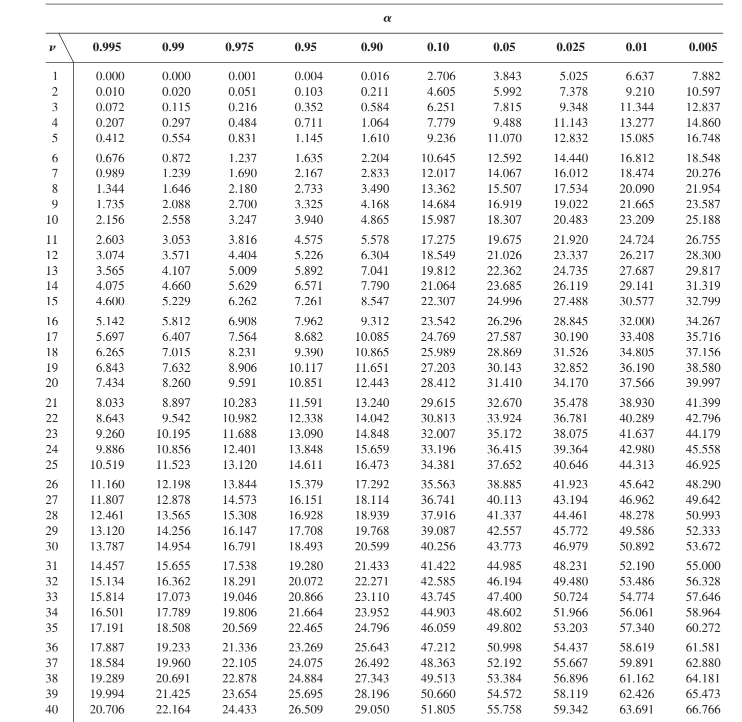
\includegraphics[width=1\linewidth]{image.png}
    \caption{Tabla de Valores Críticos de $\chi^2$. Tomado de ~\cite{devore2008}}
    \label{fig:placeholder}
\end{figure}

\vspace{-0.4cm}


\section{Material Complementario}
Se puede acceder al notebook en el que se realizo el análisis de los datos por medio del siguiente enlace:
\url{https://github.com/Jesus-Gamboa/Experimental_IV/blob/main/Medida_de_la_constante_de_Boltzman/Informe.ipynb}


\end{document}